% Figure 2: Safe-Max ROM Calibration Profile
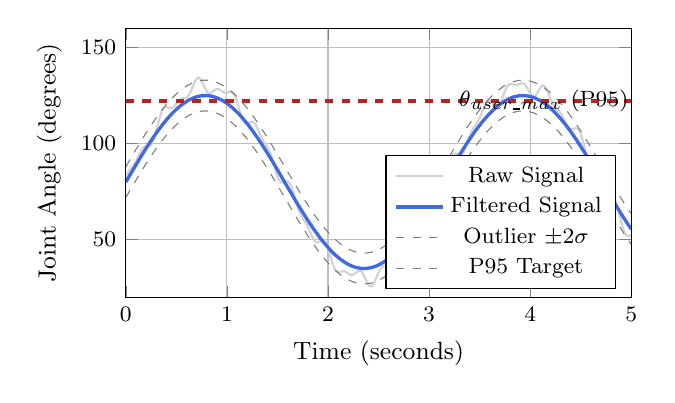
\begin{tikzpicture}
\begin{axis}[
    width=8cm, height=5cm,
    xlabel={Time (seconds)},
    ylabel={Joint Angle (degrees)},
    xmin=0, xmax=5,
    ymin=20, ymax=160,
    grid=major,
    legend pos=south east,
    legend style={font=\footnotesize},
    tick label style={font=\footnotesize},
    label style={font=\small}
]

% Raw signal with jitter
\addplot[color=LightGray, thick, domain=0:5, samples=200]
    {80 + 50*sin(deg(2*x)) + 3*sin(deg(20*x)) + 2*cos(deg(35*x))};
\addlegendentry{Raw Signal}

% Filtered signal (smooth)
\addplot[color=RoyalBlue, very thick, domain=0:5, samples=100]
    {80 + 45*sin(deg(2*x))};
\addlegendentry{Filtered Signal}

% Upper outlier boundary (+2σ)
\addplot[color=gray, dashed, domain=0:5, samples=100]
    {80 + 45*sin(deg(2*x)) + 8};
\addlegendentry{Outlier $\pm 2\sigma$}

% Lower outlier boundary (-2σ)
\addplot[color=gray, dashed, domain=0:5, samples=100]
    {80 + 45*sin(deg(2*x)) - 8};

% P95 Target ROM Threshold
\addplot[color=BrickRed, dashed, ultra thick, domain=0:5] {122};
\addlegendentry{P95 Target}

% Annotation for P95
\node[anchor=west, font=\footnotesize] at (axis cs:3.2,122) {$\theta_{\text{user\_max}}$ (P95)};

\end{axis}
\end{tikzpicture}
